\documentclass[10pt,ignorenonframetext,compress, aspectratio=169]{beamer}
\setbeamertemplate{caption}[numbered]
\setbeamertemplate{caption label separator}{: }
\setbeamercolor{caption name}{fg=normal text.fg}
\beamertemplatenavigationsymbolsempty
\usepackage{lmodern}
\usepackage{amssymb,amsmath,mathtools}
\usepackage{ifxetex,ifluatex}
\usepackage{fixltx2e} % provides \textsubscript
\ifnum 0\ifxetex 1\fi\ifluatex 1\fi=0 % if pdftex
  \usepackage[T1]{fontenc}
  \usepackage[utf8]{inputenc}
\else % if luatex or xelatex
  \ifxetex
    \usepackage{mathspec}
  \else
    \usepackage{fontspec}
  \fi
  %%\defaultfontfeatures{Ligatures=TeX,Scale=MatchLowercase}
  \defaultfontfeatures{Scale=MatchLowercase}
\fi
\usetheme[]{metropolis}
% use upquote if available, for straight quotes in verbatim environments
\IfFileExists{upquote.sty}{\usepackage{upquote}}{}
% use microtype if available
\IfFileExists{microtype.sty}{%
\usepackage{microtype}
\UseMicrotypeSet[protrusion]{basicmath} % disable protrusion for tt fonts
}{}
\newif\ifbibliography
\usepackage{graphicx,grffile}
\makeatletter
\def\maxwidth{\ifdim\Gin@nat@width>\linewidth\linewidth\else\Gin@nat@width\fi}
\def\maxheight{\ifdim\Gin@nat@height>\textheight0.8\textheight\else\Gin@nat@height\fi}
\makeatother
% Scale images if necessary, so that they will not overflow the page
% margins by default, and it is still possible to overwrite the defaults
% using explicit options in \includegraphics[width, height, ...]{}
\setkeys{Gin}{width=\maxwidth,height=\maxheight,keepaspectratio}

% Prevent slide breaks in the middle of a paragraph:
\widowpenalties 1 10000
\raggedbottom

\AtBeginPart{
  \let\insertpartnumber\relax
  \let\partname\relax
  \frame{\partpage}
}
\AtBeginSection{
  \ifbibliography
  \else
    \let\insertsectionnumber\relax
    \let\sectionname\relax
    \frame{\sectionpage}
  \fi
}
\AtBeginSubsection{
  \let\insertsubsectionnumber\relax
  \let\subsectionname\relax
  \frame{\subsectionpage}
}

\setlength{\parindent}{0pt}
\setlength{\parskip}{6pt plus 2pt minus 1pt}
\setlength{\emergencystretch}{3em}  % prevent overfull lines
\providecommand{\tightlist}{%
  \setlength{\itemsep}{0pt}\setlength{\parskip}{0pt}}
\setcounter{secnumdepth}{0}

%% GLS Added
% Textcomp for various common symbols
\usepackage{textcomp}

\usepackage{booktabs}

% Creative Commons Icons
\usepackage[scale=1]{ccicons}

\newenvironment{centrefig}{\begin{figure}\centering}{\end{figure}}
\newcommand{\columnsbegin}{\begin{columns}}
\newcommand{\columnsend}{\end{columns}}
\newcommand{\centreFigBegin}{\begin{figure}\centering}
\newcommand{\centreFigEnd}{\end{figure}}
%%


\title{Introduction}
\author{Gavin L. Simpson}
\date{February, 2017}

\begin{document}
\frame{\titlepage}

\section{Introduction}\label{introduction}

\begin{frame}{Who am I?}

\columnsbegin
\column{0.6\linewidth}

\begin{itemize}
\tightlist
\item
  Ecologist \& limnologist

  \begin{itemize}
  \tightlist
  \item
    Use palaeo as a tool
  \end{itemize}
\item
  Statistical ecologist
\item
  Not an ecological statistician
\item
  Used to teach the ``ECRC Numerical Course'' with John Birks
\item
  Now a research scientist at IECS, U Regina
\item
  Interested in

  \begin{itemize}
  \tightlist
  \item
    ecosystem response to environmental change
  \item
    community dynamics
  \item
    effects of N deposition on remote oligotrophic lakes
  \item
    effects of nutrient enrichment on prarie lakes
  \item
    C \& N dynamics
  \item
    statistical modelling
  \end{itemize}
\end{itemize}

\column{0.4\linewidth}

\begin{figure}[htbp]
\centering
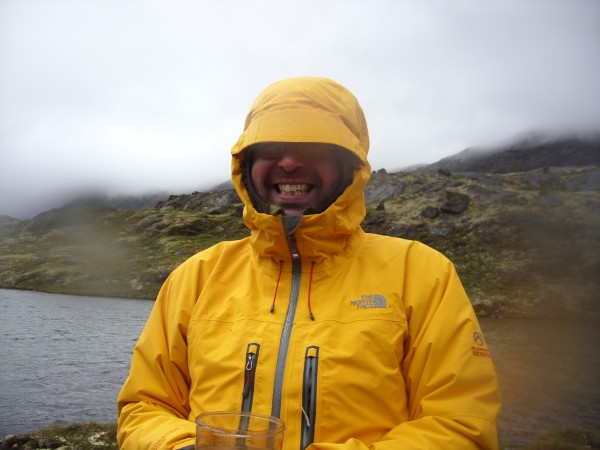
\includegraphics[width=1.00000\textwidth]{me_wet_greenland.jpg}
\caption{Me on a miserable summers day in Greenland}
\end{figure}

\columnsend

\end{frame}

\begin{frame}{Philosophy}

We want to use methods that are

\begin{itemize}
\tightlist
\item
  ecologically plausible
\item
  simple without being too simple
\item
  not unduly complex
\end{itemize}

John Birks' legacy on quantiative palaeoecology

Yet as a field we haven't moved with the times --- squandering John's
legacy

What was simple / not too complex 20 years ago may not be the best
``simple-non-complex'' way now

As a field we are crap at training

\end{frame}

\begin{frame}{Reproducibility}

Who here could reproduce the analyses for their

\begin{itemize}
\tightlist
\item
  terminal degree disertation?
\item
  last paper?
\end{itemize}

For a worrying example, see Richard Telford's blog for his ongoing
attempts to reproduce results from Lake Żabińskie (LaroqueTobler et al,
2015, \emph{QSR} \textbf{111} 35--50)

\href{https://quantpalaeo.wordpress.com/tag/larocque-tobler-et-al-2015/}{}

\end{frame}

\begin{frame}{Schedule}

Lectures 0930--1200 Lunch 1200-1300 Computers 1300--you give up

\begin{itemize}
\tightlist
\item
  Monday

  \begin{itemize}
  \tightlist
  \item
    Intro to R
  \item
    Linear models
  \end{itemize}
\item
  Tuesday

  \begin{itemize}
  \tightlist
  \item
    GLMs
  \item
    GAMs
  \end{itemize}
\item
  Wednesday

  \begin{itemize}
  \tightlist
  \item
    Ordination
  \end{itemize}
\item
  Thursday

  \begin{itemize}
  \tightlist
  \item
    Stratigraphic data
  \item
    Time series
  \end{itemize}
\item
  Friday

  \begin{itemize}
  \tightlist
  \item
    GLMMs
  \item
    Requests from the audience
  \end{itemize}
\end{itemize}

\end{frame}

\begin{frame}{Re-use}

Copyright © (2017) Gavin L. Simpson Some Rights Reserved

Unless indicated otherwise, this slide deck is licensed under a
\href{http://creativecommons.org/licenses/by/4.0/}{Creative Commons
Attribution 4.0 International License}.

\begin{center}
  \ccby
\end{center}

\end{frame}

\end{document}
